\saltoPag{} 
\section{UNIDAD 7}
    \subsection{Cinética química}
    \sangria{} Estudia las velocidades de las reacciones químicas y los mecanismos por los cuales se producen. \\
    \sangria{} Si una reacción es termodinámicamente favorable puede ocurrir, aunque no necesariamente a una velocidad observable.
    \begin{center}\scalebox{0.9}{$2{HCl}_{(ac)} + Mg{(OH)}_{2(s)} \rightleftharpoons Mg{Cl}_{2((ac))} + 2H_2O_{(l)}$} \\[2pt] \textcolor{red}{$\Delta G = -97kJ$} \end{center} \vspace{5pt}
    \begin{center} $C_{(diamante)} + O_{2(g)} \rightleftharpoons CO_{2(g)}$ \\[2pt] \textcolor{red}{$\Delta G = -396kJ$} \end{center} \vspace{5pt}
    \subsection{Velocidad de reacción}
        \sangria{} La velocidad de reacción es el cambio de la concentración de un reactivo o un producto por unidad de tiempo ($M/s$).
        \ecuacion{A \rightleftharpoons B}
        Entonces:
        \begin{center} \begin{tabular}{|m{2cm}|m{5cm}|} \toprule \multicolumn{1}{m{2cm}}{$V = - \frac{\Delta [A]}{\Delta t}$} & \multicolumn{1}{m{5cm}}{$\Delta [A] =$ cambio de concentración en $A$ respecto a un periodo de tiempo $\Delta t$.} \\ \midrule \midrule \multicolumn{1}{m{2cm}}{$V = \frac{\Delta [B]}{\Delta t}$} & \multicolumn{1}{m{5cm}}{$\Delta [B]$ = cambio de concentración en $B$ respecto a un periodo de tiempo $\Delta t$.} \\ \bottomrule \end{tabular} \end{center} 
        \imagen{6cm}{./imagenes/graficoVelocidadReaccion.png}
        \sangria{} Nótese que $[A]$ decrece con el tiempo, entonces $\Delta [A]$ es negativo. \imagen{8cm}{./imagenes/velocidadDeReaccionProceso.png}
        \textbf{\underline{Ejemplo:}} \\[5pt] \scalebox{0.9}{$Br_{2(ac)} + HCOOH_{(ac)} \rightleftharpoons {2Br^-}_{(ac)} + {2H^+}_{(ac)} + {CO}_{2(g)}$} \columnbreak{} \imagen{7cm}{./imagenes/boroReaccion.png} \ecuacion{\underrightarrow{\text{\textit{\hspace{15pt}Tiempo\hspace{15pt}}}}} \vspace{5pt} \imagen{7cm}{./imagenes/transparenciaBoro.png} Moles de $Br_2$ a lo largo del tiempo: \imagen{8cm}{./imagenes/pendienteMolesBr2Tiempo.png}
        \begin{center} \begin{tabular}{|m{1.5cm}|m{6.5cm}|} \toprule \multicolumn{1}{|m{2cm}|}{\textbf{Velocidad promedio}} & \multicolumn{1}{m{6cm}|}{$-\frac{\Delta [Br_2]}{\Delta t} = - \frac{[Br_2]_{final} - [Br_2]_{inicial}}{t_{final} - t_{inicial}}$} \\ \midrule \multicolumn{1}{|m{2cm}|}{\textbf{Velocidad instantánea}} & \multicolumn{1}{m{6cm}|}{Velocidad en un tiempo específico.} \\ \bottomrule \end{tabular} \end{center} 
        \imagen{8cm}{./imagenes/velocidadesBrEnElTiempo.png}
        \begin{center} \begin{tabular}{|m{8cm}|} \toprule \multicolumn{1}{|m{8cm}|}{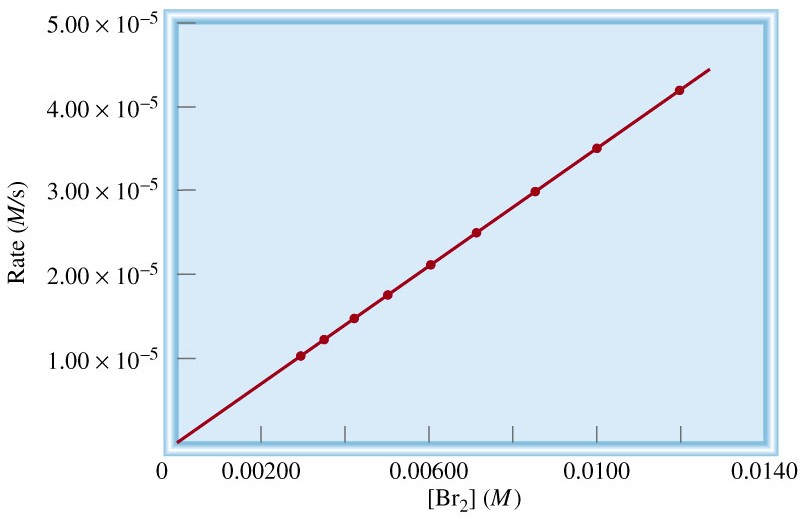
\includegraphics[width=7cm]{./imagenes/rectaMolesTiempoDelBoro.png}} \\ \midrule \multicolumn{1}{|m{8cm}|}{$Velocidad \propto [Br_2]$} \\[2pt] \multicolumn{1}{|m{8cm}|}{$Velocidad = k[Br_2]$} \\[2pt] \multicolumn{1}{|m{8cm}|}{$k = \frac{V}{[Br_2]}$} \\[5pt] \multicolumn{1}{|m{8cm}|}{$k \approx 3,50 \times 10^{-3} s^{-1}$} \\ \bottomrule \end{tabular} \end{center}
        \saltoPag{}
        \midTitle{blue}{Medir $\Delta P$ respecto al tiempo}
        \imagen{3cm}{./imagenes/medirVariacionPresionRespectoAlTiempo.png}
        Siendo: \ecuacion{2H_2O_{2(ac)} \rightleftharpoons 2H_2O_{(l)} + O_{2(g)}} \begin{center} $PV = nRT$ \\[2pt] $P = \frac{n}{V}RT = [O_2]RT$ \\ $[O_2] = \frac{1}{RT}P$ \\[3pt] \recuadrar{5cm}{$Veloc = \frac{\Delta [O_2]}{\Delta t} = \frac{1}{RT} \frac{\Delta P}{\Delta t}$} \end{center} \imagen{6cm}{./imagenes/variacionPresionRespectoAlTiempoGrafico.png}
    \subsubsection{Estequiometría}
        \ecuacion{2A \rightleftharpoons B}
        \sangria{} Dos moles de $A$ desaparecen por cada mol de $B$ que se forme.
        \ecuacion{V = \unMedio \frac{\Delta [A]}{\Delta t} \hspace{15pt} V = \frac{\Delta [B]}{\Delta t}}
        \ecuacion{aA + bB \rightleftharpoons cC + dD}
        \recuadrar{7cm}{$V = - \frac{1}{a}\frac{\Delta [A]}{\Delta t} = - \inv{b} \frac{\Delta [B]}{\Delta t} = \inv{c} \frac{\Delta [C]}{\Delta t} = \inv{d}\frac{\Delta [D]}{\Delta t}$} \imagen{8cm}{./imagenes/ejemploVelocidadReaccion.png}
    \subsubsection{Ley de la velocidad}
        \sangria{} La ley de la velocidad expresa el producto de la concentración de los reactivos elevados a una potencia llamada \textbf{orden de reacción}.
        \ecuacion{aA + bB \rightleftharpoons cC + dD}
        \recuadrar{4cm}{$V = k [A]^x[B]^y$}
        Siendo:
        \begin{itemize}
            \item La reacción es el orden $x$ respecto a $A$.
            \item La reacción es de orden $y$ respecto a $B$.
            \item La reacción general es de orden $(x+y)$.
        \end{itemize}
    \textbf{\underline{Ejemplo:}} \ecuacion{F_{2(g)} + 2ClO_{2(g)} \rightleftharpoons 2FClO_{2(g)}} \ecuacion{\text{Ley de velocidad:}\hspace{5pt} V = k[F_2]^x[ClO_2]^y} \imagen{7cm}{./imagenes/experimentosParaLeyDeVelocidad.png} \begin{center} \textit{Experimentos para determinar los órdenes} \end{center} Razonando: \begin{itemize} \item Duplicando $[F_2]$ con $[ClO_2]$ constante, la velocidad se duplica. Por lo tanto $X=1$. \item Cuadruplicando $[ClO_2]$ con $[F_2]$ constante, la velocidad se aumenta 4 veces. Por lo tanto $Y=1$. \end{itemize} Resultado: \recuadrar{4cm}{$V = k[F_2][ClO_2]$} La reacción es de orden $1$ con respecto a $F_2$. \\ La reacción es de orden $1$ con respecto a $ClO_2$. \\ El orden global de la reacción es de $2$.
    \saltoPag{}
    \midTitle{blue}{Leyes de la velocidad}\begin{itemize} \item Las leyes de la velocidad son determinadas experimentalmente. \item El orden de la reacción siempre es definido en términos de las concentraciones del reactivo (no del producto). \item La orden de un reactivo no esa relacionado con el coeficiente estequiométrico del reactivo en la ecuación química balanceada. \end{itemize}
    \subsubsection{Determinación experimental de la ecuación de velocidad}
    Siendo: \ecuacion{CH_3-Cl_{(g)} + H_2O_{(g)} \rightleftharpoons CH_3-OH_{(g)} + HCl_{(g)}} \imagen{6cm}{./imagenes/determinacionExperimentalEcuacionVelocidad.png} Usando los datos de la tabla: \ecuacion{V = k [CH_3-Cl][H_2O]^2} \ecuacion{k = \frac{V}{[CH_3-Cl][H_2O]^2} = 181,12 \inv{M^2\cdot S}}
        \textbf{\underline{Otro ejemplo:}} \\[2pt] \sangria{} Considere una reacción química entre los compuestos $A$ y $B$, que es de primer orden respecto de $A$ y de segundo orden respecto de $B$. De la información dada abajo complete los espacios en blanco: \ecuacion{V = k [A][B]^2} \begin{center} \begin{tabular}{|m{2cm}|m{2cm}|m{1cm}|m{1cm}|} \toprule \multicolumn{1}{|c}{Experimento} & \multicolumn{1}{c}{Velocidad($M/s$)} & \multicolumn{1}{c}{$[A]$} & \multicolumn{1}{c|}{$[B]$} \\ \midrule \multicolumn{1}{|c}{1} & \multicolumn{1}{c}{$0,150$} & \multicolumn{1}{c}{$1,00M$} & \multicolumn{1}{c|}{$0,200M$} \\ \multicolumn{1}{|c}{2} & \multicolumn{1}{c}{$0,3$} & \multicolumn{1}{c}{$2,00M$} & \multicolumn{1}{c|}{$0,200M$} \\ \multicolumn{1}{|c}{3} & \multicolumn{1}{c}{$1,2$} & \multicolumn{1}{c}{$2,00M$} & \multicolumn{1}{c|}{$0,400M$} \\ \bottomrule \end{tabular} \end{center} \ecuacion{0,1500 M/s = k[1M][0,2M]^2} \recuadrar{5cm}{$ k = 3,75 \inv{M^2\cdot S}$} 
        \midTitle{red}{Reacciones de orden cero} Para la reacción del tipo $A \rightarrow productos$ \ecuacion{V = k[A]^0 \Longrightarrow k} \begin{center} \begin{tabular}{|c|c|c|} \toprule \multicolumn{1}{|c}{\textbf{Orden}} & \multicolumn{1}{c}{\textbf{Ley de velocidad}} & \multicolumn{1}{c|}{\textbf{Unidades de $K$}} \\ \midrule \multicolumn{1}{|c}{0} & \multicolumn{1}{c}{$v = k$} & \multicolumn{1}{c|}{$M/s$} \\[5pt] \multicolumn{1}{|c}{1} & \multicolumn{1}{c}{$v = k[A]$} & \multicolumn{1}{c|}{$\inv{s}$} \\[5pt] \multicolumn{1}{|c}{2} & \multicolumn{1}{c}{$v = k[A]^2$} & \multicolumn{1}{c|}{$\inv{M\cdot s}$} \\[5pt] \bottomrule \end{tabular} \end{center}
        \columnbreak{}
        \subsection{Teoría de las colisiones - Energía de activación ($E_A$)}
    \sangria{} El número de moléculas de productos es proporcional al número de choques entre las moléculas de los reactivos. \\ \sangria{} De éstos choques, no todos son efectivos, porque: \begin{itemize} \item no tienen la energía necesaria para constituir el ''complejo activado''. \item no tienen la orientación adecuada. \end{itemize} \sangria{} La energía de activación es la necesaria para formar el ''complejo activado'', a partir del cual la reacción transcurre de forma natural. \imagen{7cm}{./imagenes/orientacionEnElChoque.png} \ecuacion{A + B \rightarrow {AB^+}^+ \rightarrow C + D} \imagen{7cm}{./imagenes/energiaDeActivacionReaccionesEndoExo.png} \sangria{} La energía de activación ($E_A$) es la energía mínima requerida para iniciar una reacción.
    \midTitle{red}{Perfil de una reacción} \imagen{8cm}{./imagenes/perfilDeUnaReaccion.png}
    \subsection{Ecuación de Arrhenius - Dependencia de la constante de velocidad con la temperatura}
\recuadrar{5cm}{$k = A \cdot e ^{\frac{E_A}{RT}}$} \saltoPag{} Siendo: \begin{itemize} \item $k$: constante de velocidad. \item $E_A$: energía de activación ($kJ/mol$) \item $A$: factor de frecuencia de colisiones. \item $R$: constante de los gases ideales. \item $T$: temperatura absoluta. \end{itemize} Normalmente se encuentra expresa en su forma logarítmica para calcular $E_A$: \ecuacion{\ln k = \ln A - \frac{E_A}{RT}} \imagen{5cm}{./imagenes/temperaturaVSConstanteVelocidad.png}
    \subsection{Catalizadores}
\sangria{} Intervienen en alguna etapa de la reacción pero no se modifican pues se recuperan al final y no aparece en la ecuación global ajustada. \\ \sangria{} Modifican el mecanismo y por tanto $E_A$. \sangria{} Las reacciones catalizadas también pueden clasificarse en: \begin{itemize} \item Homogéneos: en la misma fase que los reactivos. \item Heterogéneos: se encuentran en distinta fase. \end{itemize} \sangria{} Un catalizador (positivo) es una sustancia que incrementa la velocidad de la reacción disminuyendo la energía de activación. \imagen{7cm}{./imagenes/catalizadorPositivo.png} 
    \subsubsection{Catálisis heterogénea}

    \imagen{6cm}{./imagenes/catalisisHeterogenea.png} \sangria{} En una catálisis heterogénea, los reactivos y el catalizador están en diferentes fases. \begin{itemize} \item Síntesis de Haber para el amoniaco. \item Proceso de Ostwald para la producción de ácido nítrico. \item Convertidores catalíticos. \end{itemize} 
    \midTitle{red}{Proceso Haber} \imagen{6cm}{./imagenes/procesoHaber.png} \ecuacion{N_{2(g)} + 3H_{2(g)} \hspace{10pt} \underrightarrow{Fe/Al_2O_3/K_2O 500^oC} \hspace{10pt} 2NH_{3(g)}} \vspace{-20pt} \begin{center} \hspace{20pt}catalizador \end{center}
    \midTitle{red}{Proceso Ostwald} \begin{center} Pt-Rh catalizador $800^oC$ \end{center} \ecuacion{4NH_{3(g)} + 5O_{2(g)} \rightarrow 4NO_{(g)} + 6H_2O_{(g)}} \ecuacion{2NO_{(g)} + O_{2(g)} \rightarrow 2NO_{2(g)}} \ecuacion{2NO_{2(g)} + H_2O_{(l)} \rightarrow HNO_{2(ac)} + HNO_{3(ac)}} \imagen{4cm}{./imagenes/catalizadoresUsadosProcesoOstwald.png} \begin{center} \textit{Catalizadores Pt-Rh usados en el proceso Ostwald} \end{center} \imagen{3cm}{./imagenes/alambreCalientePtSobreSolucionNH3.png}
    \subsubsection{Catálisis homogénea}
\sangria{} En una catálisis homogénea, los reactivos y el catalizador están dispersos en una sola fase, por lo regular líquida. \begin{itemize} \item Catálisis ácida. \item Catálisis básica o alcalina. \end{itemize} \saltoPag{}
    \subsubsection{Convertidores catalíticos}
        \imagen{8cm}{./imagenes/convertidorCatalitico.png}


